\documentclass[11pt]{article}
\usepackage[a4paper,margin=1.8cm]{geometry}
\usepackage{fontspec}
\usepackage{xeCJK}
\usepackage{unicode-math}
\setmainfont{texgyretermes-regular.otf}[
  Path=/usr/share/texlive/texmf-dist/fonts/opentype/public/tex-gyre/,
  BoldFont=texgyretermes-bold.otf,
  ItalicFont=texgyretermes-italic.otf,
  BoldItalicFont=texgyretermes-bolditalic.otf
]
\setsansfont{texgyreheros-regular.otf}[
  Path=/usr/share/texlive/texmf-dist/fonts/opentype/public/tex-gyre/,
  BoldFont=texgyreheros-bold.otf,
  ItalicFont=texgyreheros-italic.otf,
  BoldItalicFont=texgyreheros-bolditalic.otf
]
\setmonofont{lmmono10-regular.otf}[
  Path=/usr/share/texlive/texmf-dist/fonts/opentype/public/lm/,
  ItalicFont=lmmono10-italic.otf
]
\setmathfont{texgyretermes-math.otf}[
  Path=/usr/share/texlive/texmf-dist/fonts/opentype/public/tex-gyre-math/
]
\setCJKmainfont{FandolSong-Regular.otf}[
  Path=/users/a/e/aereinh/render_resources/chinese_math_pdf/texmf/fonts/opentype/public/fandol/,
  BoldFont=FandolSong-Bold.otf,
  AutoFakeSlant=0.18
]
\setCJKsansfont{FandolHei-Regular.otf}[
  Path=/users/a/e/aereinh/render_resources/chinese_math_pdf/texmf/fonts/opentype/public/fandol/,
  BoldFont=FandolHei-Bold.otf
]
\setCJKmonofont{FandolSong-Regular.otf}[
  Path=/users/a/e/aereinh/render_resources/chinese_math_pdf/texmf/fonts/opentype/public/fandol/,
  BoldFont=FandolSong-Bold.otf
]
\usepackage{graphicx}
\usepackage{longtable}
\usepackage{booktabs}
\usepackage{xcolor}
\usepackage{hyperref}
\hypersetup{colorlinks=true,linkcolor=blue,urlcolor=blue}
\setlength{\parindent}{0pt}
\setlength{\parskip}{0.55em}
\begin{document}
\begin{titlepage}
\centering
{\Huge CARE Myocardium 失败取证 Deep Research 证据包\par}
\vspace{1cm}
{\Large 20260730 本地证据冻结版\par}
\vfill
本 PDF 是可搜索中文报告。它不是新模型蓝图，不包含 validation upload，也不声明 hosted 指标。
\end{titlepage}
\tableofcontents
\clearpage
\section*{一页执行摘要}
这轮取证的直接结论是：当前最可靠的动作不是继续设计新 CARE 架构，而是先把评价语义、checkpoint/recipe 绑定、病例级统一重聚合、PRISM decoder-reset 对照、MoSAIC recipe decomposition 和 Cine temporal probe 做成可复现证据。已确认的硬边界是 pure edema 与 edema-zone 不能混写，full-data MoSAIC 不能冒充 clean fold0，pending 或未跑完的 GPU 诊断不能写成科学完成。

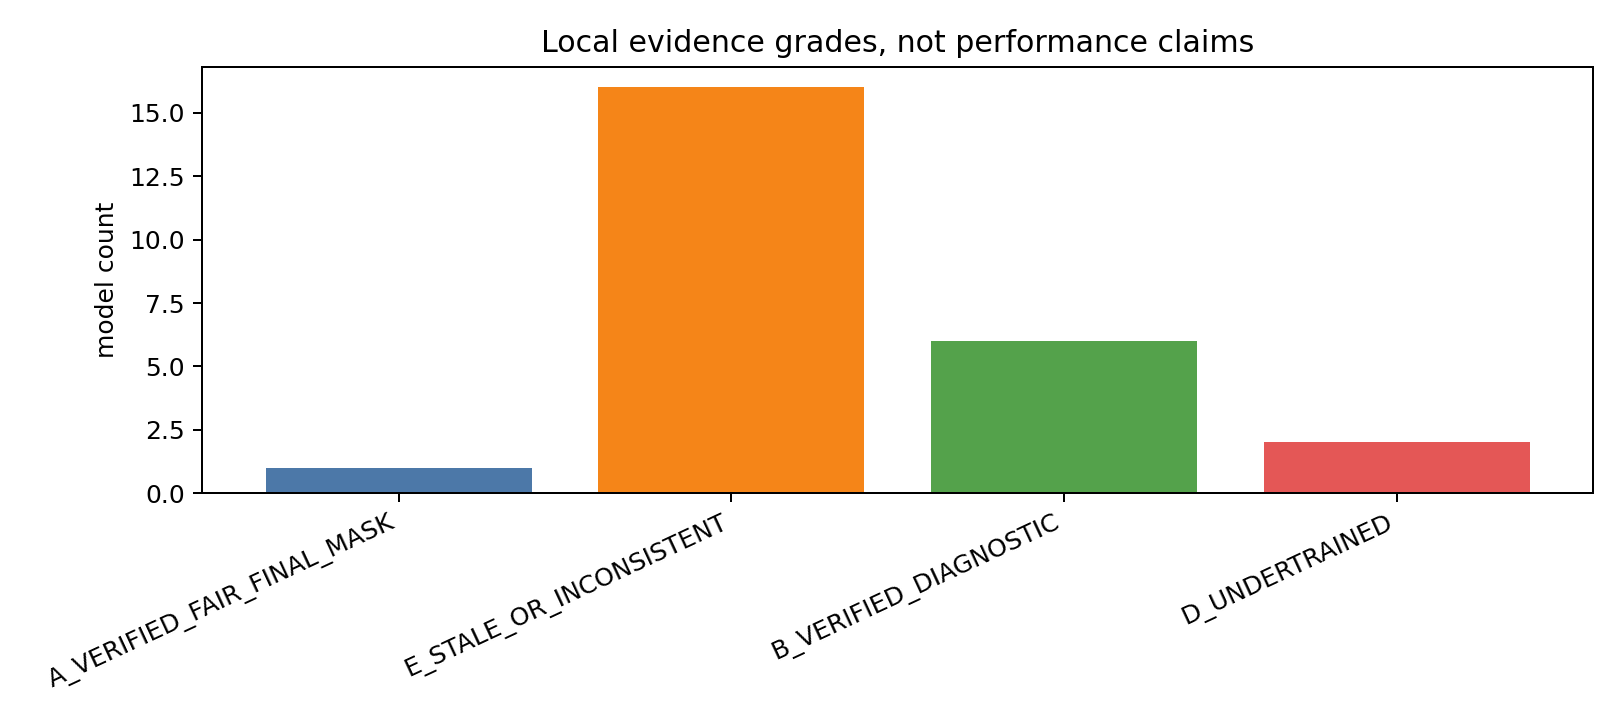
\includegraphics[width=0.95\linewidth]{generated_figures/evidence_grade_counts.png}
\clearpage
\input{sections/section_01.tex}
\section{2. CARE 数据、中心、模态和标签真值}

本章先回答一个取证问题：现有本地证据能否支持对应的科学判断。它重要是因为过去多条路线混合了设计承诺、实现状态、训练预算、评价语义和 hosted 结果。本包只采用本地可绑定证据；无法绑定的数字不会被写成性能结论。



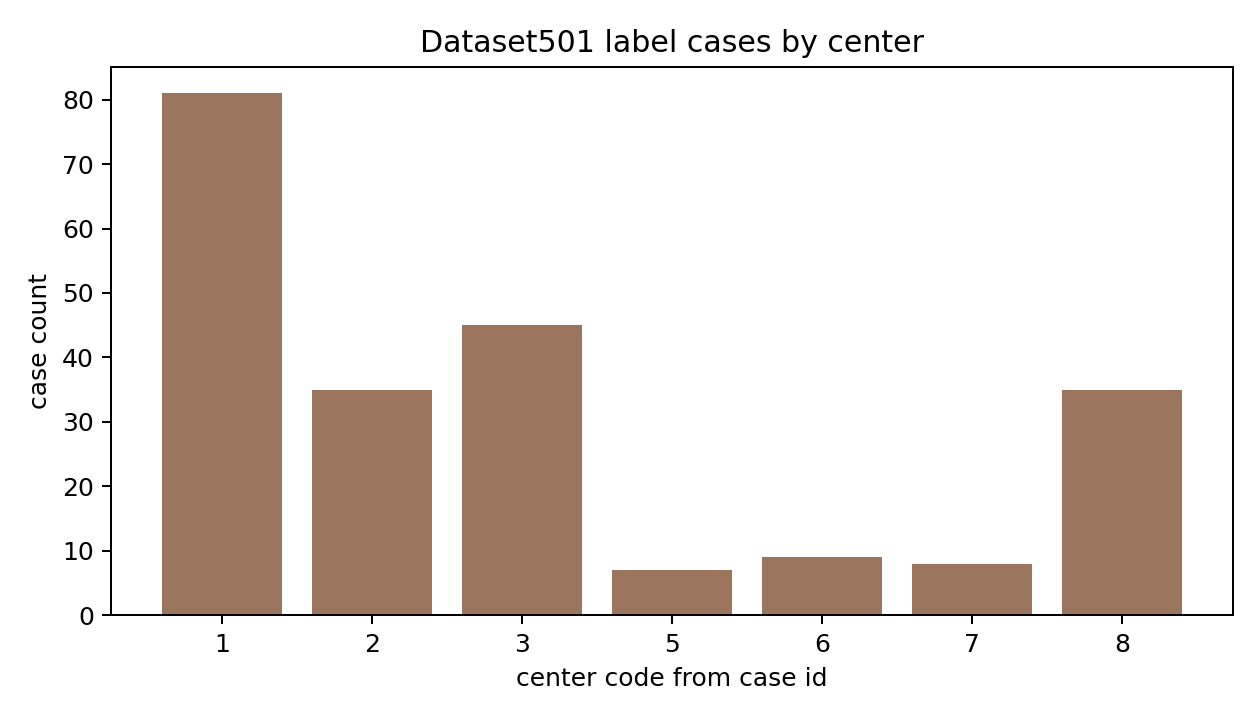
\includegraphics[width=0.92\linewidth]{generated_figures/center_case_counts.png}

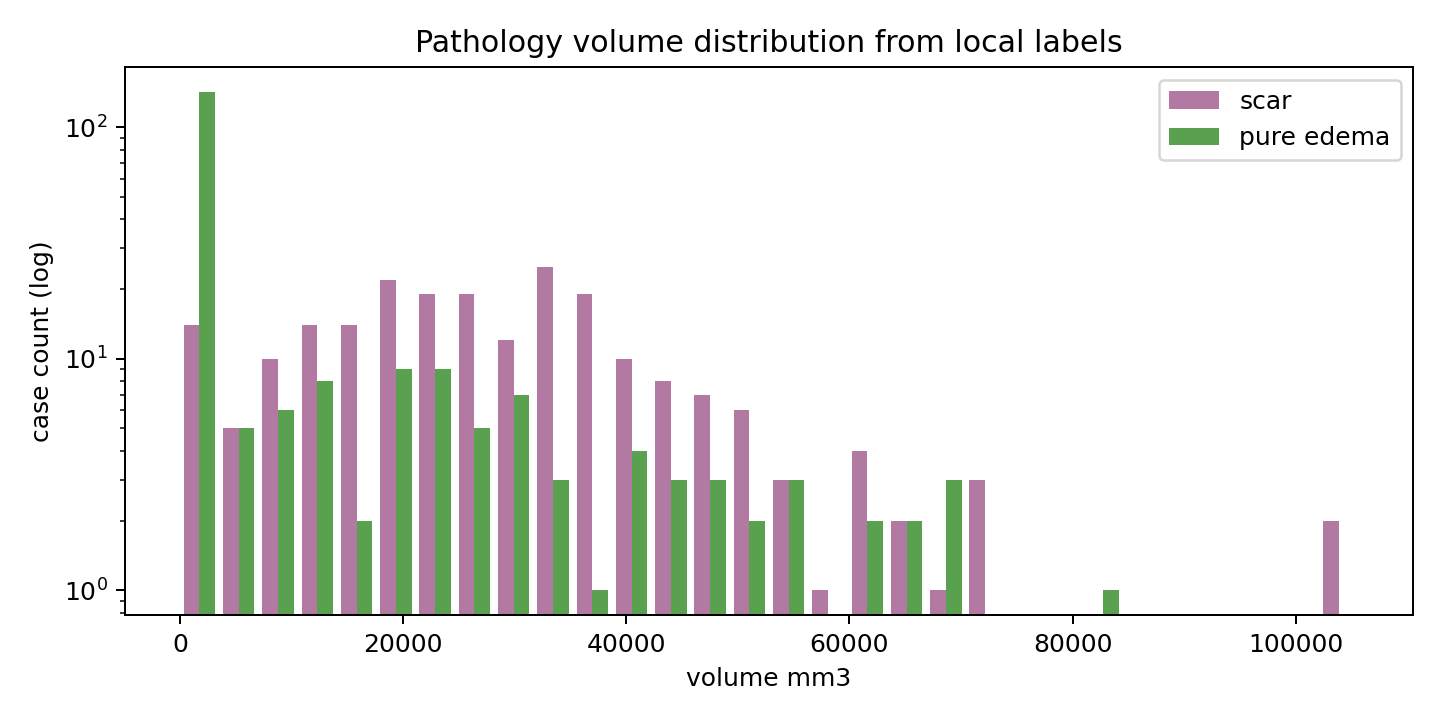
\includegraphics[width=0.92\linewidth]{generated_figures/pathology_volume_distribution.png}

\begin{longtable}{p{0.19\linewidth}p{0.19\linewidth}p{0.19\linewidth}p{0.19\linewidth}p{0.19\linewidth}}
\toprule
cases & scar\_positive & pure\_edema\_positive & t2\_present\\
\midrule
220 & 212 & 80 & 220\\
\bottomrule
\end{longtable}



\clearpage
\section{3. 官方与内部指标语义}

本章先回答一个取证问题：现有本地证据能否支持对应的科学判断。它重要是因为过去多条路线混合了设计承诺、实现状态、训练预算、评价语义和 hosted 结果。本包只采用本地可绑定证据；无法绑定的数字不会被写成性能结论。



\begin{longtable}{p{0.19\linewidth}p{0.19\linewidth}p{0.19\linewidth}p{0.19\linewidth}p{0.19\linewidth}}
\toprule
object & internal\_labels & official\_export & allowed\_claim\_scope\\
\midrule
scar & 5 & scar & official\\
pure\_edema & 4 & edema & T2-present official edema\\
edema\_zone & 4|5 & none & internal only\\
\bottomrule
\end{longtable}

关键边界：[E-METRIC-001] known-bad fixture 已覆盖 spacing HD95、empty case、remote FP 和 label 4/5 混淆。



\clearpage
\input{sections/section_04.tex}
\section{5. nnU-Net 强基线到底强在哪里}

本章先回答一个取证问题：现有本地证据能否支持对应的科学判断。它重要是因为过去多条路线混合了设计承诺、实现状态、训练预算、评价语义和 hosted 结果。本包只采用本地可绑定证据；无法绑定的数字不会被写成性能结论。



nnU-Net 仍是现代强基线。当前包不以 foreground mean 掩盖 scar 和 pure edema；统一重聚合尚未完成。

\begin{longtable}{p{0.19\linewidth}p{0.19\linewidth}p{0.19\linewidth}p{0.19\linewidth}p{0.19\linewidth}}
\toprule
model\_id & design\_goal & input\_modalities & missing\_modality\_handling & backbone\\
\midrule
NNUNET & historical CARE route or baseline & UNBOUND\_OR\_ROUTE\_SPECIFIC & UNBOUND & UNBOUND\\
SRR\_V2 & historical CARE route or baseline & UNBOUND\_OR\_ROUTE\_SPECIFIC & UNBOUND & UNBOUND\\
SRR\_V25 & historical CARE route or baseline & UNBOUND\_OR\_ROUTE\_SPECIFIC & UNBOUND & UNBOUND\\
SRR\_V3 & historical CARE route or baseline & UNBOUND\_OR\_ROUTE\_SPECIFIC & UNBOUND & UNBOUND\\
BATCH0 & historical CARE route or baseline & UNBOUND\_OR\_ROUTE\_SPECIFIC & UNBOUND & UNBOUND\\
\bottomrule
\end{longtable}



\clearpage
\input{sections/section_06.tex}
\input{sections/section_07.tex}
\input{sections/section_08.tex}
\input{sections/section_09.tex}
\input{sections/section_10.tex}
\section{11. PRISM W1-W3 的完整复盘}

本章先回答一个取证问题：现有本地证据能否支持对应的科学判断。它重要是因为过去多条路线混合了设计承诺、实现状态、训练预算、评价语义和 hosted 结果。本包只采用本地可绑定证据；无法绑定的数字不会被写成性能结论。



PRISM 不能只看是否有强 encoder。D0-D3 未完成前，不能判断低分主要来自 representation、decoder reset 还是训练协议。

\begin{longtable}{p{0.19\linewidth}p{0.19\linewidth}p{0.19\linewidth}p{0.19\linewidth}p{0.19\linewidth}}
\toprule
diagnostic & status\\
\midrule
D0\_FULL\_PRETRAINED\_IDENTITY & NOT\_RUN\\
\bottomrule
\end{longtable}



\clearpage
\section{12. MoSAIC clean、full-data 和 hosted recipe}

本章先回答一个取证问题：现有本地证据能否支持对应的科学判断。它重要是因为过去多条路线混合了设计承诺、实现状态、训练预算、评价语义和 hosted 结果。本包只采用本地可绑定证据；无法绑定的数字不会被写成性能结论。



MoSAIC 必须拆成 clean fold0、full-data diagnostic 和 hosted-near recipe 三层。full-data 权重不能作为 clean architecture 比较。

\begin{longtable}{p{0.19\linewidth}p{0.19\linewidth}p{0.19\linewidth}p{0.19\linewidth}p{0.19\linewidth}}
\toprule
status\\
\midrule
NOT\_RUN\\
\bottomrule
\end{longtable}



\clearpage
\input{sections/section_13.tex}
\input{sections/section_14.tex}
\section{15. case-wise help/harm}

本章先回答一个取证问题：现有本地证据能否支持对应的科学判断。它重要是因为过去多条路线混合了设计承诺、实现状态、训练预算、评价语义和 hosted 结果。本包只采用本地可绑定证据；无法绑定的数字不会被写成性能结论。



当前证据边界：本章只作为 Deep Research 的定位层，完整病例级重算或 GPU 诊断仍需后续 terminal wave。



\clearpage
\section{16. 失败病例视觉图册}

本章先回答一个取证问题：现有本地证据能否支持对应的科学判断。它重要是因为过去多条路线混合了设计承诺、实现状态、训练预算、评价语义和 hosted 结果。本包只采用本地可绑定证据；无法绑定的数字不会被写成性能结论。



病例 montage 的选择依赖 standardized_casewise_metrics。本包目前只生成 QA contact sheet，明确标注 VISUAL_HUMAN_CONFIRMATION_PENDING。



\clearpage
\input{sections/section_17.tex}
\section{18. selector feasibility}

本章先回答一个取证问题：现有本地证据能否支持对应的科学判断。它重要是因为过去多条路线混合了设计承诺、实现状态、训练预算、评价语义和 hosted 结果。本包只采用本地可绑定证据；无法绑定的数字不会被写成性能结论。



若 selector nested CV 不能稳定超过 always-best-single-model，必须写 LOCAL_EVIDENCE_DOES_NOT_SUPPORT_DEPLOYABLE_MODEL_SELECTION。当前 selector 尚未运行。



\clearpage
\input{sections/section_19.tex}
\section{20. decoder-reset 诊断对照}

本章先回答一个取证问题：现有本地证据能否支持对应的科学判断。它重要是因为过去多条路线混合了设计承诺、实现状态、训练预算、评价语义和 hosted 结果。本包只采用本地可绑定证据；无法绑定的数字不会被写成性能结论。



\begin{longtable}{p{0.19\linewidth}p{0.19\linewidth}p{0.19\linewidth}p{0.19\linewidth}p{0.19\linewidth}}
\toprule
diagnostic & status\\
\midrule
D0-D3 & NOT\_RUN\\
\bottomrule
\end{longtable}



\clearpage
\input{sections/section_21.tex}
\input{sections/section_22.tex}
\input{sections/section_23.tex}
\section{24. Cine 的真实瓶颈}

本章先回答一个取证问题：现有本地证据能否支持对应的科学判断。它重要是因为过去多条路线混合了设计承诺、实现状态、训练预算、评价语义和 hosted 结果。本包只采用本地可绑定证据；无法绑定的数字不会被写成性能结论。



Cine temporal signal 必须用 patient-level P0 ED-only 与 P1 temporal probe 对照。本包没有把单帧输出冒充 temporal evidence。



\clearpage
\input{sections/section_25.tex}
\section{26. 根因排序与证据图}

本章先回答一个取证问题：现有本地证据能否支持对应的科学判断。它重要是因为过去多条路线混合了设计承诺、实现状态、训练预算、评价语义和 hosted 结果。本包只采用本地可绑定证据；无法绑定的数字不会被写成性能结论。



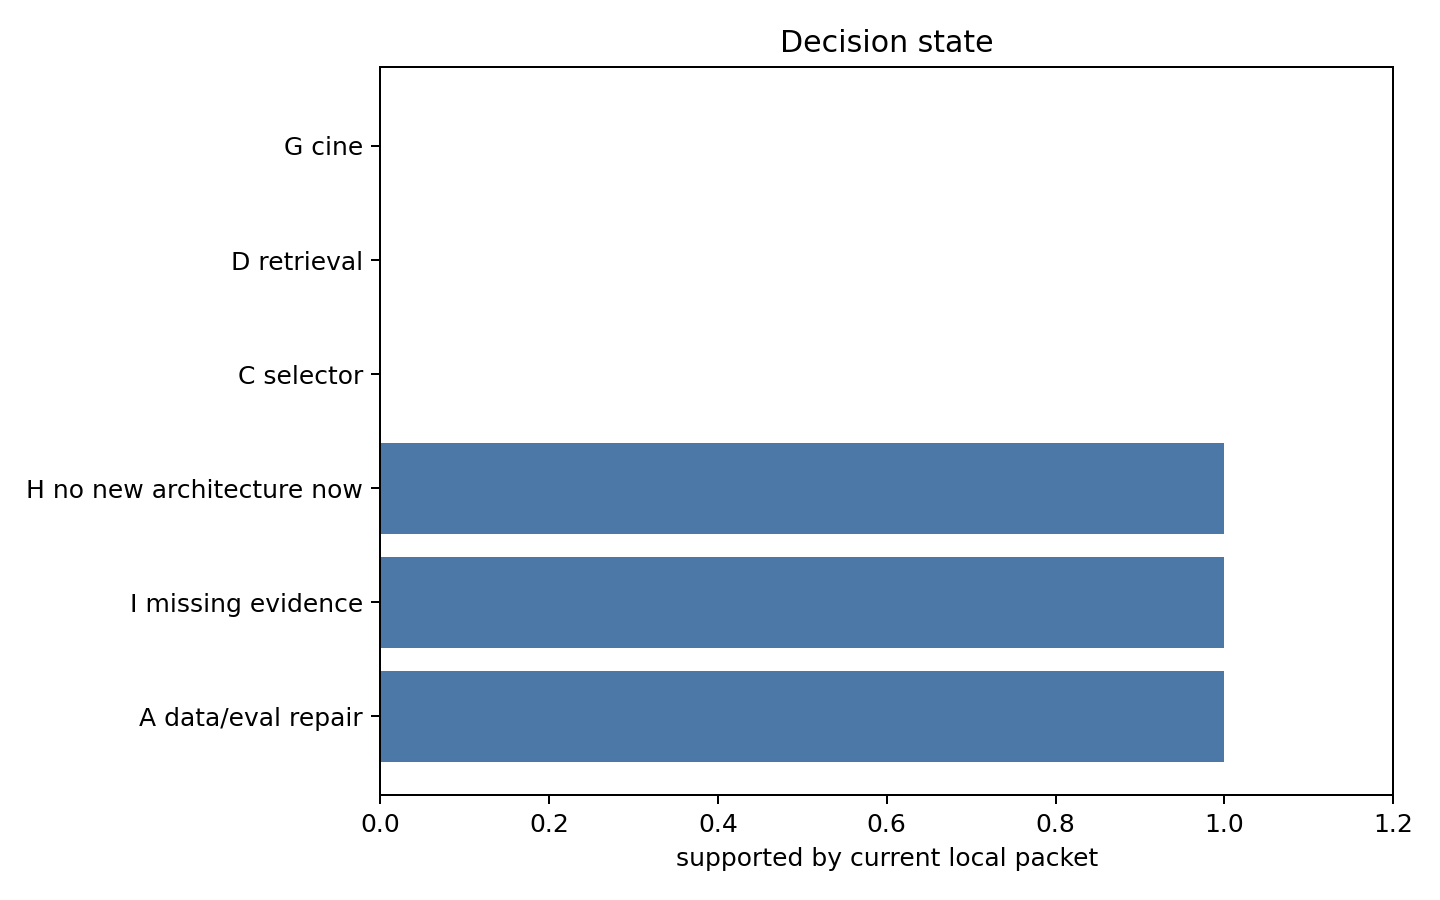
\includegraphics[width=0.92\linewidth]{generated_figures/decision_state.png}

\begin{longtable}{p{0.19\linewidth}p{0.19\linewidth}p{0.19\linewidth}p{0.19\linewidth}p{0.19\linewidth}}
\toprule
root\_cause & evidence & counterevidence & affected\_models & affected\_pathology\\
\midrule
METRIC\_IMPLEMENTATION & remote FP 和 pure-edema/edema-zone 语义已有 known-bad 保护；全量影响未重算。 & not yet fully tested & multiple & scar|pure\_edema|cine\\
CHECKPOINT\_OR\_RECIPE & MoSAIC clean/full-data/hosted recipe 未绑定完成，存在本地证据反转风险。 & not yet fully tested & multiple & scar|pure\_edema|cine\\
DECODER\_CAPABILITY\_LOSS & PRISM decoder-reset 假说合理但 D0-D3 未运行。 & not yet fully tested & multiple & scar|pure\_edema|cine\\
COMPONENT\_NOT\_WIRED & 多个路线需 forward/on-off 才能确认模块是否进入 final logits。 & not yet fully tested & multiple & scar|pure\_edema|cine\\
INSUFFICIENT\_PATHOLOGY\_SIGNAL & feature probe 未运行。 & not yet fully tested & multiple & scar|pure\_edema|cine\\
MULTIMODAL\_MISALIGNMENT & alignment correlation 未运行。 & not yet fully tested & multiple & scar|pure\_edema|cine\\
CINE\_TASK\_DEFINITION & Cine P0/P1 未运行。 & not yet fully tested & multiple & scar|pure\_edema|cine\\
\bottomrule
\end{longtable}



\clearpage
\section{27. 当前能下的结论}

本章先回答一个取证问题：现有本地证据能否支持对应的科学判断。它重要是因为过去多条路线混合了设计承诺、实现状态、训练预算、评价语义和 hosted 结果。本包只采用本地可绑定证据；无法绑定的数字不会被写成性能结论。



# Local Evidence Conclusions

当前本地证据支持 A 和 I：先做评价/数据/recipe 绑定修复，并承认关键证据仍缺失。尚不能支持新的 CARE 架构蓝图。




\clearpage
\section{28. 当前不能下的结论}

本章先回答一个取证问题：现有本地证据能否支持对应的科学判断。它重要是因为过去多条路线混合了设计承诺、实现状态、训练预算、评价语义和 hosted 结果。本包只采用本地可绑定证据；无法绑定的数字不会被写成性能结论。



当前不能下的结论：不能声称任何新架构已被支持；不能声称 MoSAIC clean 天然强于 nnU-Net；不能声称 alignment 或 Cine temporal 是主因。



\clearpage
\section{29. 外部 Deep Research 必须回答的问题}

本章先回答一个取证问题：现有本地证据能否支持对应的科学判断。它重要是因为过去多条路线混合了设计承诺、实现状态、训练预算、评价语义和 hosted 结果。本包只采用本地可绑定证据；无法绑定的数字不会被写成性能结论。



- [DR-001] Small-lesion scar segmentation beyond nnU-Net requires which evidence standard?
- [DR-002] Can clean MoSAIC recipe gains be separated from full-data target-domain advantage?
- [DR-003] Do frozen encoder features contain patient-held-out scar FN/FP separability?
- [DR-004] When does cine temporal information improve pathology segmentation over ED-only?




\clearpage
\section{30. 下一轮决策树}

本章先回答一个取证问题：现有本地证据能否支持对应的科学判断。它重要是因为过去多条路线混合了设计承诺、实现状态、训练预算、评价语义和 hosted 结果。本包只采用本地可绑定证据；无法绑定的数字不会被写成性能结论。



# Research Decision Tree

1. 先完成 evaluation/data repair。
2. 若 D0 不能复现 nnU-Net，停止 decoder-reset。
3. 若 selector nested CV 不超过 always-best-single-model，停止 deployable selector。
4. 若 feature probe control 不成立，停止 retrieval/prototype 叙事。




\clearpage
\appendix
\section{模型和 checkpoint provenance}
\begin{longtable}{p{0.19\linewidth}p{0.19\linewidth}p{0.19\linewidth}p{0.19\linewidth}p{0.19\linewidth}}
\toprule
model\_id & path & size\_bytes & sha256 & hash\_status\\
\midrule
NNUNET & /users/a/e/aereinh/CARE/data/nnUNet/nnUNet\_results/Dataset502\_CARECineMyoPS/nnUNetTrainer\_\_nnUNetPlans\_\_3d\_fullres/fold\_0/checkpoint\_final.pth & 354608437 &  & LARGE\_METADATA\_ONLY\\
NNUNET & /users/a/e/aereinh/CARE/data/nnUNet/nnUNet\_results/Dataset502\_CARECineMyoPS/nnUNetTrainer\_\_nnUNetPlans\_\_3d\_fullres/fold\_0/checkpoint\_best.pth & 354266799 &  & LARGE\_METADATA\_ONLY\\
NNUNET & /users/a/e/aereinh/CARE/data/nnUNet/nnUNet\_results/Dataset502\_CARECineMyoPS/nnUNetTrainer\_500epochs\_\_nnUNetPlans\_\_3d\_fullres/fold\_4/checkpoint\_final.pth & 354383029 &  & LARGE\_METADATA\_ONLY\\
NNUNET & /users/a/e/aereinh/CARE/data/nnUNet/nnUNet\_results/Dataset502\_CARECineMyoPS/nnUNetTrainer\_500epochs\_\_nnUNetPlans\_\_3d\_fullres/fold\_4/checkpoint\_best.pth & 354382767 &  & LARGE\_METADATA\_ONLY\\
NNUNET & /users/a/e/aereinh/CARE/data/nnUNet/nnUNet\_results/Dataset502\_CARECineMyoPS/nnUNetTrainer\_500epochs\_\_nnUNetPlans\_\_3d\_fullres/fold\_0/checkpoint\_final.pth & 354382965 &  & LARGE\_METADATA\_ONLY\\
NNUNET & /users/a/e/aereinh/CARE/data/nnUNet/nnUNet\_results/Dataset502\_CARECineMyoPS/nnUNetTrainer\_500epochs\_\_nnUNetPlans\_\_3d\_fullres/fold\_0/checkpoint\_best.pth & 354201839 &  & LARGE\_METADATA\_ONLY\\
NNUNET & /users/a/e/aereinh/CARE/data/nnUNet/nnUNet\_results/Dataset502\_CARECineMyoPS/nnUNetTrainer\_500epochs\_\_nnUNetPlans\_\_3d\_fullres/fold\_2/checkpoint\_final.pth & 354383093 &  & LARGE\_METADATA\_ONLY\\
NNUNET & /users/a/e/aereinh/CARE/data/nnUNet/nnUNet\_results/Dataset502\_CARECineMyoPS/nnUNetTrainer\_500epochs\_\_nnUNetPlans\_\_3d\_fullres/fold\_2/checkpoint\_best.pth & 354242031 &  & LARGE\_METADATA\_ONLY\\
NNUNET & /users/a/e/aereinh/CARE/data/nnUNet/nnUNet\_results/Dataset502\_CARECineMyoPS/nnUNetTrainer\_500epochs\_\_nnUNetPlans\_\_3d\_fullres/fold\_1/checkpoint\_final.pth & 354383349 &  & LARGE\_METADATA\_ONLY\\
NNUNET & /users/a/e/aereinh/CARE/data/nnUNet/nnUNet\_results/Dataset502\_CARECineMyoPS/nnUNetTrainer\_500epochs\_\_nnUNetPlans\_\_3d\_fullres/fold\_1/checkpoint\_best.pth & 354270127 &  & LARGE\_METADATA\_ONLY\\
NNUNET & /users/a/e/aereinh/CARE/data/nnUNet/nnUNet\_results/Dataset502\_CARECineMyoPS/nnUNetTrainer\_500epochs\_\_nnUNetPlans\_\_3d\_fullres/fold\_3/checkpoint\_final.pth & 354382965 &  & LARGE\_METADATA\_ONLY\\
NNUNET & /users/a/e/aereinh/CARE/data/nnUNet/nnUNet\_results/Dataset502\_CARECineMyoPS/nnUNetTrainer\_500epochs\_\_nnUNetPlans\_\_3d\_fullres/fold\_3/checkpoint\_best.pth & 354369135 &  & LARGE\_METADATA\_ONLY\\
NNUNET & /users/a/e/aereinh/CARE/data/nnUNet/nnUNet\_results/nnUNet/2d/Task025\_Cine\_Seg/nnUNetTrainerV2\_\_nnUNetPlansv2.1/fold\_0/model\_final\_checkpoint.model.pkl & 31579 & ea87fb6002a766379c529eaf0c56107113e17861efefac4e7b54d81c0ea5cc0b & PREFIX\_8192\_BYTES\\
NNUNET & /users/a/e/aereinh/CARE/data/nnUNet/nnUNet\_results/nnUNet/2d/Task025\_Cine\_Seg/nnUNetTrainerV2\_\_nnUNetPlansv2.1/fold\_0/model\_final\_checkpoint.model & 235538772 &  & LARGE\_METADATA\_ONLY\\
NNUNET & /users/a/e/aereinh/CARE/data/nnUNet/nnUNet\_results/nnUNet/2d/Task026\_Cine\_4D\_smoke/CARECineMyoPSTrainer\_\_nnUNetPlansv2.1/fold\_0/model\_final\_checkpoint.model.pkl & 4305 & cdeca70da84be8d8db3471352c0728f073ab4ac911cff1ba34104206c565c5e9 & FULL\\
NNUNET & /users/a/e/aereinh/CARE/data/nnUNet/nnUNet\_results/nnUNet/2d/Task026\_Cine\_4D\_smoke/CARECineMyoPSTrainer\_\_nnUNetPlansv2.1/fold\_0/model\_final\_checkpoint.model & 1669319383 &  & LARGE\_METADATA\_ONLY\\
NNUNET & /users/a/e/aereinh/CARE/results/20260726\_care\_fullinfo\_nnunet\_and\_care\_scf/care\_scf\_v1/mosaic\_oof\_checkpoint\_manifest.csv & 1985 & b9ffabd601e3e9a502a4cf9be4fb602de6029a0688591c7d39cf05af21683e09 & FULL\\
NNUNET & /users/a/e/aereinh/CARE/results/20260726\_care\_fullinfo\_nnunet\_and\_care\_scf/care\_scf\_v1/mosaic\_oof/fold0/oof\_checkpoint\_manifest.csv & 441 & 86bdeb34e4b90695dcdcac41e55461ca912f060fccba84f8717a99d1cbdf2850 & FULL\\
NNUNET & /users/a/e/aereinh/CARE/data/nnUNet/nnUNet\_results/nnUNet/2d/Task026\_Cine\_4D/CARECineMyoPSTrainer\_\_nnUNetPlansv2.1/fold\_0/model\_final\_checkpoint.model.pkl & 68222 & 39b3eea294b9e0b04fee593f69189e461d29b7f64ed4a13fd2c7579f7b64792e & PREFIX\_8192\_BYTES\\
NNUNET & /users/a/e/aereinh/CARE/data/nnUNet/nnUNet\_results/nnUNet/2d/Task026\_Cine\_4D/CARECineMyoPSTrainer\_\_nnUNetPlansv2.1/fold\_0/model\_final\_checkpoint.model & 1669390615 &  & LARGE\_METADATA\_ONLY\\
\bottomrule
\end{longtable}
\section{指标公式和 known-bad}
\begin{longtable}{p{0.19\linewidth}p{0.19\linewidth}p{0.19\linewidth}p{0.19\linewidth}p{0.19\linewidth}}
\toprule
claim\_id & claim\_text & pdf\_page & section & source\_path\\
\midrule
E-DATA-001 & 本包读取 Dataset501 labelsTr 的病例清单并统计标签体积。 &  & 2 & data\_case\_manifest.csv\\
E-METRIC-001 & reference metric known-bad fixtures pass for remote FP, spacing HD95, empty cases and lesion recall. &  & 3 & reference\_metric\_known\_bad\_report.json\\
E-MOSAIC-001 & full-data MoSAIC evidence cannot be used as clean fold0 comparison. &  & 12 & mosaic\_ablation\_contract.json\\
E-PRISM-001 & PRISM decoder-reset explanation remains unresolved until D0-D3 terminal diagnostics complete. &  & 20 & decoder\_reset\_diagnostic\_report.md\\
E-GAP-005 & Required diagnostic evidence item 5 remains incomplete and is not used as a performance claim. &  & 5 & strict\_validator\_report.json\\
E-GAP-006 & Required diagnostic evidence item 6 remains incomplete and is not used as a performance claim. &  & 6 & strict\_validator\_report.json\\
E-GAP-007 & Required diagnostic evidence item 7 remains incomplete and is not used as a performance claim. &  & 7 & strict\_validator\_report.json\\
E-GAP-008 & Required diagnostic evidence item 8 remains incomplete and is not used as a performance claim. &  & 8 & strict\_validator\_report.json\\
E-GAP-009 & Required diagnostic evidence item 9 remains incomplete and is not used as a performance claim. &  & 9 & strict\_validator\_report.json\\
E-GAP-010 & Required diagnostic evidence item 10 remains incomplete and is not used as a performance claim. &  & 10 & strict\_validator\_report.json\\
E-GAP-011 & Required diagnostic evidence item 11 remains incomplete and is not used as a performance claim. &  & 11 & strict\_validator\_report.json\\
E-GAP-012 & Required diagnostic evidence item 12 remains incomplete and is not used as a performance claim. &  & 12 & strict\_validator\_report.json\\
E-GAP-013 & Required diagnostic evidence item 13 remains incomplete and is not used as a performance claim. &  & 13 & strict\_validator\_report.json\\
E-GAP-014 & Required diagnostic evidence item 14 remains incomplete and is not used as a performance claim. &  & 14 & strict\_validator\_report.json\\
E-GAP-015 & Required diagnostic evidence item 15 remains incomplete and is not used as a performance claim. &  & 15 & strict\_validator\_report.json\\
E-GAP-016 & Required diagnostic evidence item 16 remains incomplete and is not used as a performance claim. &  & 16 & strict\_validator\_report.json\\
E-GAP-017 & Required diagnostic evidence item 17 remains incomplete and is not used as a performance claim. &  & 17 & strict\_validator\_report.json\\
E-GAP-018 & Required diagnostic evidence item 18 remains incomplete and is not used as a performance claim. &  & 18 & strict\_validator\_report.json\\
E-GAP-019 & Required diagnostic evidence item 19 remains incomplete and is not used as a performance claim. &  & 19 & strict\_validator\_report.json\\
E-GAP-020 & Required diagnostic evidence item 20 remains incomplete and is not used as a performance claim. &  & 20 & strict\_validator\_report.json\\
\bottomrule
\end{longtable}
\section{证据缺口}
本附录列出所有 strict validator 阻断项，防止后续误读为完成。

\end{document}
